\section{Linear Programming Optimization}

Linear programming is a commonly used techniques in optimization. In linear programming, we want to optimize (maximize or minimize) a linear function, subject to a set of linear inequalities (called linear constraints). 

\begin{definition}[Linear Constraint] \index{linear function} \index{linear equality} \index{linear inequality} \index{linear constraint}
    Given a set of real numbers $a_1,a_2,\ldots,a_n$ and a set of variables $x_1,x_2,\ldots,x_n$, a \textit{\textbf{linear function}} $f$ on those variables is
    $$
    f(x_1,\ldots,x_n) = a_1x_1 + a_2x_2 + \cdots + a_nx_n = \sum_{j=1}^n a_jx_j
    $$
    If $b$ is a real number and $f$ is a linear function, then $f(x_1,\ldots,x_n) = b$ is a linear equality ,and $(x_1,\ldots,x_n) \leq b$ and $(x_1,\ldots,x_n) \geq b$ are linear inequalities. Both linear equalities and linear inequalities are called \textit{\textbf{linear constraints}}.
\end{definition}

Geometrically, a linear function forms a line in $\R^n$. A linear inequality forms a half-space in $\R^n$. All possible solutions to a linear program lies in a convex region called the \textit{\textbf{feasible region}}. If no such region exsits (no solution satisfies all the contraints), we say the optimization problem is \textit{\textbf{infeasible}}. The function we wish to optimize is called the \textit{\textbf{objective function}}, and the value of the objective function evaluated at a particular point is called the \textit{\textbf{objective value}} at that point. The goal of the linear programming problem is to find a feasible solution that maximizes/minimizes the objective value.

\begin{theorem}[Feasible Region for Linear Programming is Convex]
    Let $\mathbf{x}_1,\mathbf{x}_2 \in \R^n$ be two feasible solutions to the linear programming problem, satisfying some particular constraints. Then, for all $\lambda \in [0,1]$, $\lambda\mathbf{x}_1 + (1-\lambda)\mathbf{x}_2$ is also a solution that satisfies the same constraints.
\end{theorem}

\begin{proof}
    Without loss of generality, suppose that the constraints are given as a system of linear equations $\mathbf{A}\mathbf{x} = \mathbf{b}$. Let $\lambda \in [0,1]$ be arbitrary.
    $$
    \begin{aligned}
        \mathbf{A}(\lambda\mathbf{x}_1 + (1-\lambda)\mathbf{x}_2) &= \lambda\mathbf{A}\mathbf{x}_1 + \mathbf{A}\mathbf{x}_2 - \lambda\mathbf{A}\mathbf{x}_2 \\
        &= \lambda \mathbf{b} + \mathbf{b} - \lambda \mathbf{b} \\
        &= \mathbf{b}
    \end{aligned}
    $$
    Hence, $\lambda\mathbf{x}_1 + (1-\lambda)\mathbf{x}_2$ is also a solution to the system of linear equation and thus is a feasible solution.
\end{proof}

Figure \ref{fig:lp-feasible-region} shows a geometric representation of a linear programming problem with the objective function $x_1+x_2$.

\begin{figure}[htbp]
    \centering
    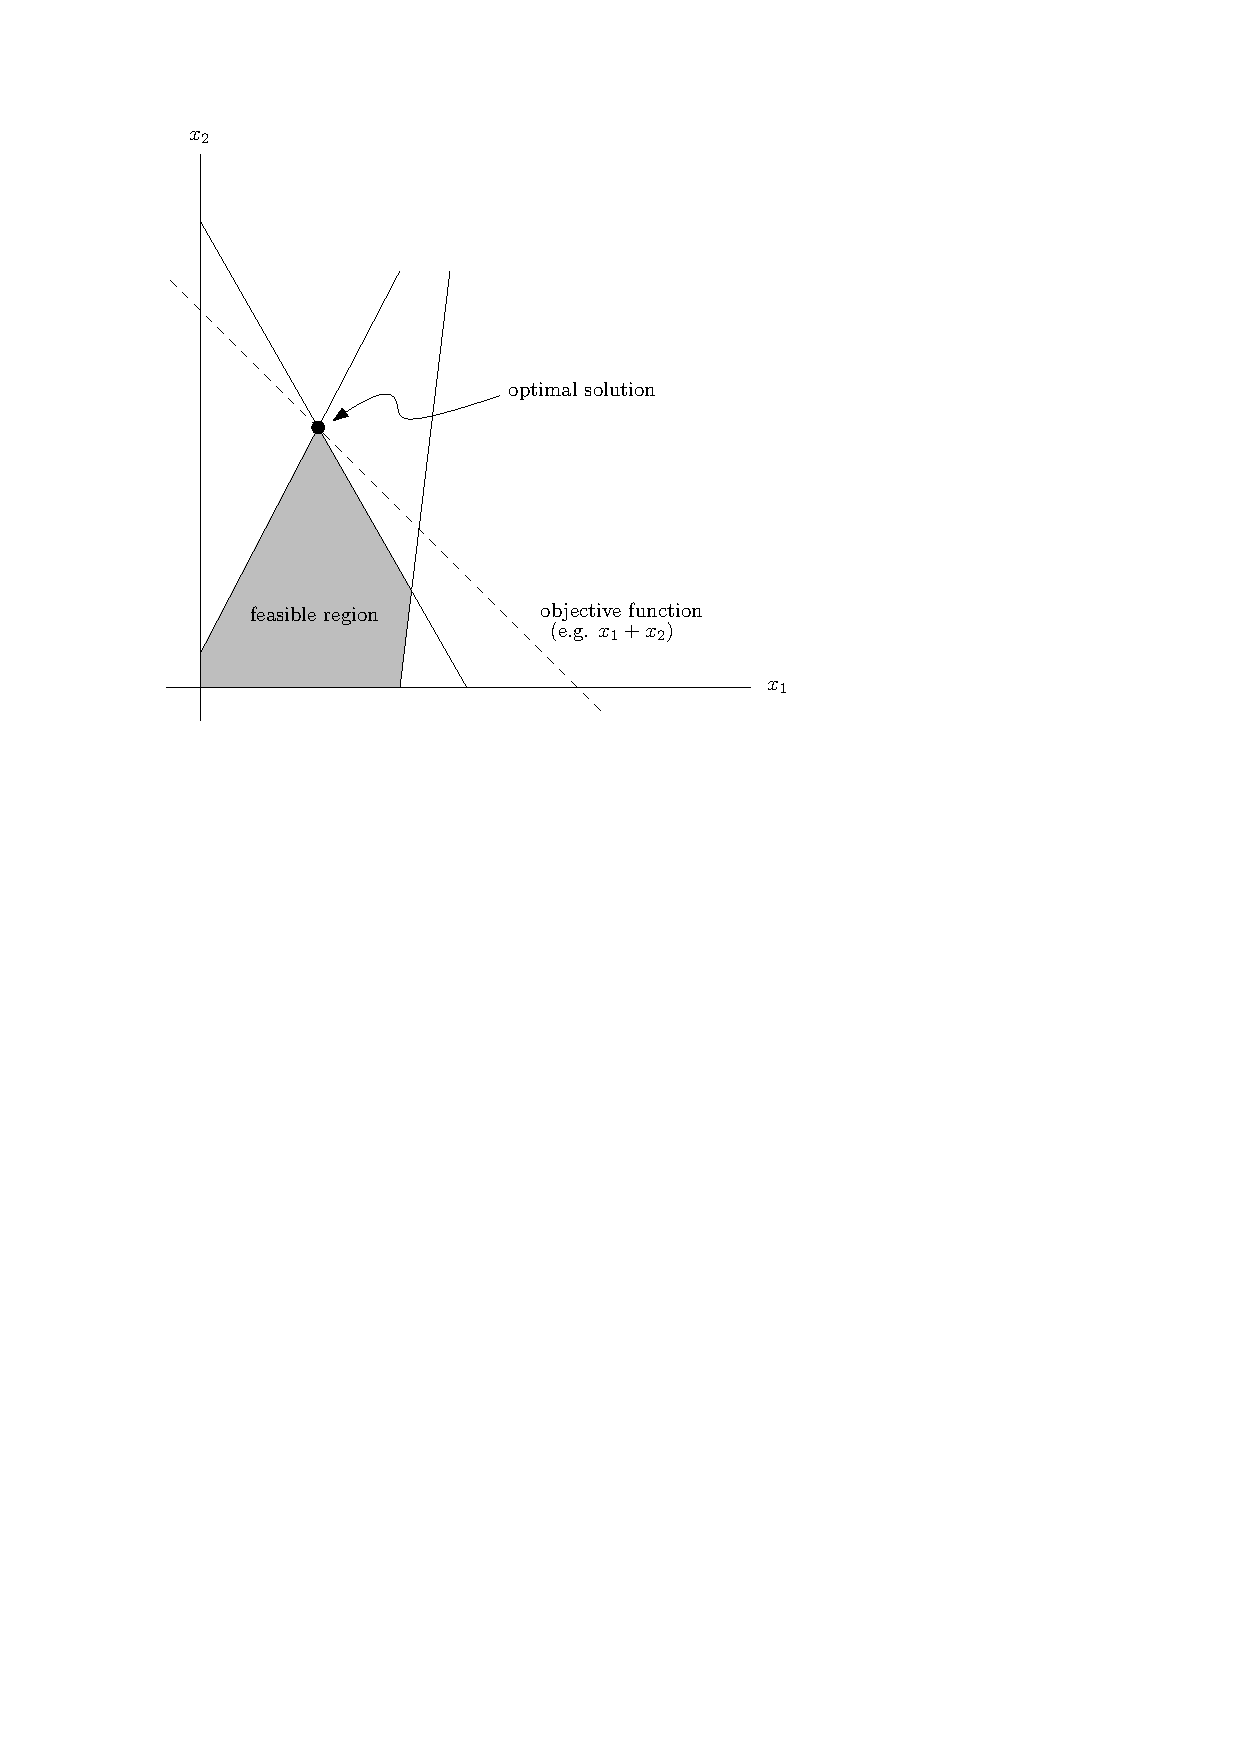
\includegraphics[width=0.5\linewidth]{lp/lp-feasible-region.pdf}
    \caption{A linear programming problem with 2 variables, 4 linear constraints (solid lines), and objective function $x_1+x_2$ (dashed line).}
    \label{fig:lp-feasible-region}
\end{figure}

\section{Standard and Slack Forms}

\subsection{Standard Form}

In standard form, we are given $n$ real numbers $c_1,\ldots,c_n$, $m$ real numbers $b_1,\ldots,b_m$, and $mn$ real numbers $a_{ij}$ for $i \in \{1,\ldots,m\}$ and $j \in \{1,\ldots,n\}$. We wish to

Maximize $\displaystyle \sum_{j=1}^n c_j x_j$ \\
Subject to
\[
    \begin{aligned}
        \sum_{j=1}^n a_{ij} x_j &\leq b_1 & \text{for $i = 1,\ldots,m$} \\
        x_j &\geq 0 & \text{for $j = 1,\ldots,n$}
    \end{aligned}
\]

or, equivalently, in vectorized form

Maximize $\mathbf{c}^\top \mathbf{x}$ \\
Subject to $\mathbf{A}\mathbf{x} \leq \mathbf{b}$ and $\mathbf{x} \geq \boldsymbol{0}$,

where $\mathbf{c}$ is an $n$-vector, $\mathbf{x}$ is an $n$-vector, $\mathbf{b}$ is an $m$-vector, and $\mathbf{A}$ is an $m \times n$ matrix. This can also be written in as a tuple $(\mathbf{A},\mathbf{b},\mathbf{c})$ as a shorthand.

This vectorized form is often used in machine learning because vectorized operations can be carried out more quickly using the GPU.

\subsection{Conversion From Non-standard Form to Standard Form}

A linear programming problem might not be in standard form, but it is easy to convert from non-standard form to standard form.

If \begin{itemize}
    \item the objective is minimization rather than maximization $\Rightarrow$ flip the sign of coefficients;
    \item there are variables without nonnegativity constraints $\Rightarrow$ say a variable $x_j$ does not have  nonnegativity constraints, replace $x_j$ with $x_j' - x_j''$ and add constraints $x_j' \geq 0$ and $x_j'' \geq 0$;
    \item the constraints are equality constraints rather than $\leq$ $\Rightarrow$ replace the constraint with two non-strict inequality constraints ($\leq$ and $\geq$);
    \item the constraints are in the opposite direction ($\geq$ instead of $\leq$) $\Rightarrow$ multiply both sides by -1 
\end{itemize}

\subsection{Slack Form}

Maximize $\displaystyle z = v + \sum_{j=1}^n c_j x_j$ \\
Subject to
\[
    \begin{aligned}
        s_i &= b_1 - \sum_{j=1}^n a_{ij} x_j & \text{for $i = 1,\ldots,m$} \\
        x_j,s_i &\geq 0 & \text{for $j = 1,\ldots,n$ and $i = 1,\ldots,m$ }
    \end{aligned}
\]

or, equivalently, in vectorized form

Maximize $z = v + \mathbf{c}^\top \mathbf{x}$ \\
Subject to $\mathbf{s} = \mathbf{b} - \mathbf{A}\mathbf{x}$ and $\mathbf{x},\mathbf{s} \geq \boldsymbol{0}$.

We call the variables on the left-hand side of the equality constraints the \textit{\textbf{basic variables}}, and the ones on the right-hand side the \textit{\textbf{non-basic variables}}.

Similarly, a slack from can be concisely defined by a tuple $(N,B,\mathbf{A},\mathbf{b},\mathbf{c},v)$, where $N$ is the set of indices of the non-basic variables, $B$ is the set of indices of the basic variables such that $|N| = n$, $|B|=m$ and $N \cup B = \{1,2,\ldots,n+m\}$.

It is called the slack from because the variable $s_i$ (or in vectorized form $\mathbf{s}$) measures remaining ``slack'' or difference between two sides of the original inequality constraints. This is related to the simplex algorithm where we increase the non-basic variables as much as possible until we hit a bottleneck -- having no more slack for that non-basic variable.

\section{Geometry of Linear Programming}

Consider the following system of inequalities
$$
\begin{aligned}
    x_1 + x_2 + x_3 &\leq 1 \\
    x_1,x_2,x_3 &\geq 0
\end{aligned}
$$
This is the type of inequalities that we often encounter in linear programming problems. The points that satisfy these inequalities forms a 3D polytope.

\begin{figure}[htbp]
    \centering
    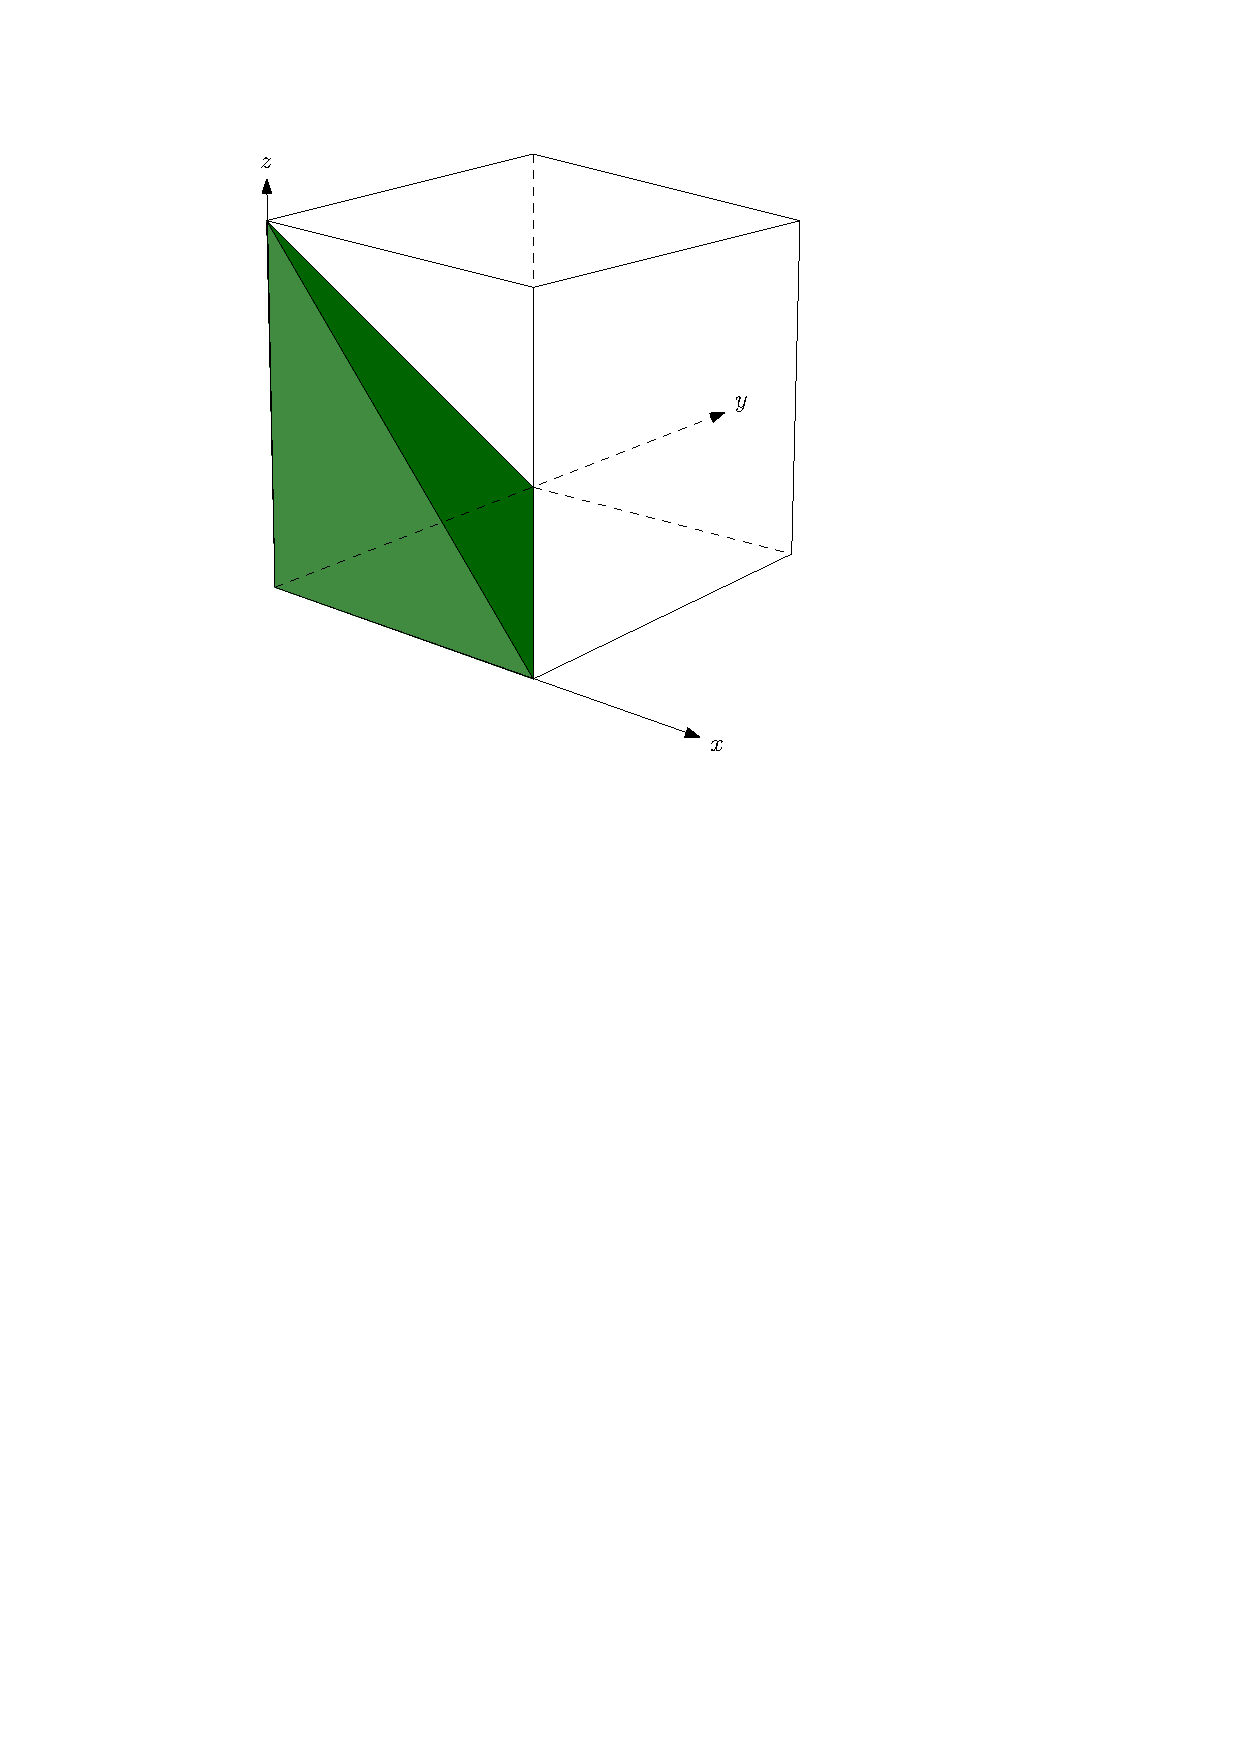
\includegraphics[width=0.4\linewidth]{lp/3d-polytope.pdf}
    \caption{A 3D polytope.}
    \label{fig:3d-polytope}
\end{figure}

\subsection{Hyperplane and Halfspace} \index{hyperplane} \index{halfspace} \index{supporting hyperplane}
In general, the set $\{ x \in \R^n \mid a^\top x = b \}$ is called a hyperplane. For all lines in the \textit{\textbf{hyperplane}} $H = \{ x \in \R^n \mid a^\top = b \}$ that intersects the line $\ell = \{ta \mid t \in \R\}$, the line is also perpendicular to $\ell$. As a simple example, consider the two-dimensional case where $a = [1\;\;-1]^\top$.

The set $\{ \mathbf{x} \in \R^n \mid \mathbf{a}^\top \mathbf{x} \leq b \}$ is called a \textit{\textbf{halfspace}}, and $\{ \mathbf{x} \in \R^n \mid \mathbf{a}^\top \mathbf{x} = b \}$ is called the \textit{\textbf{supporting hyperplane}}.

\subsection{Polyhedron and Polytope} \index{polyhedron} \index{polytope} \index{face} \index{facet}

A set that is the intersection of halfspaces is called a \textit{\textbf{polyhedron}}. A polyhedron can be defined as $\{x \in \R^n \mid \mathbf{A}\mathbf{x} \leq \mathbf{b} \}$ for some matrix $\mathbf{A}$ and vector $\mathbf{b}$.

A polyhedron $P \subseteq \R^n$ is unbounded if there exists a point $\mathbf{x} \in P$ and a direction $\mathbf{v} \in \R^n$ such that for every $t \geq 0$, $\mathbf{x} + t \mathbf{v} \in P$. If a polyhedron is bounded, we call it a \textit{\textbf{polytope}}.

A \textit{\textbf{face}} of a polyhedron $P = \{\mathbf{x} \in \R^n \mid \mathbf{A}\mathbf{x} \leq \mathbf{b} \}$ is a set $F = \{ \mathbf{x} \in \R^n \mid \mathbf{A}\mathbf{x} \leq b \} \cap \{ \mathbf{x} \in \R^n \mid \forall i \in S.\, \mathbf{a}_i \mathbf{x} = \mathbf{b}_i \}$ where $\mathbf{a}_i$ is a row vector denoting the $i$th row of matrix $\mathbf{A}$, and $S$ is some subset of the rows of $\mathbf{A}$. Intuitively, a face of a polyhedron is just one of its surface.

Assuming that $F \neq \emptyset$, we define $S_F$ to be the set of all $i \in S$ such that $\mathbf{a}_i \mathbf{x} = \mathbf{b}_i$ for all $\mathbf{x} \in F$ (we can intutively think this as the rows of constraints that created the face $F$). Let $\mathbf{A}_F$ be the submatrix of $\mathbf{A}$ containing rows of $A$ indexed by $S_F$. If the rank of $\mathbf{A}_F$ is $n-j$, we say $F$ is a face of \textit{\textbf{dimension}} $j$, or a $j$-face. The dimension of a polytope can be defined similarly. Faces of dimension one lower than the dimension of $P$ are called \textit{\textbf{facets}}, faces of dimension 1 are called \textit{\textbf{edges}}, faces of dimension 0 are called \textit{\textbf{vertices}}.

\subsection{Convex Hull}

A polytope can be determined by its vertices.

\begin{definition}[Convex Hull] \index{convex hull}
    The \textit{\textbf{convex hull}} of the points $\mathbf{v}_1,\ldots,\mathbf{v}_n \in \R^n$ is defined as the set
    $$
    \mathrm{conv} \{\mathbf{v}_1,\ldots,\mathbf{v}_n\} = \{ \lambda_1 \mathbf{v}_1 + \cdots + \lambda_n \mathbf{v}_n \mid \forall i \in \{1,\ldots,n\}.\, \lambda_i \geq 0,\; \lambda_1+\cdots+\lambda_n = 1 \}
    $$
    In general, the convex hull is the smallest polytope containing $\mathbf{v}_1,\ldots,\mathbf{v}_n$.
\end{definition}

\begin{theorem} \label{thm:convex-hull-polytope}
    A polytope $P$ with vertices $\mathbf{v}_1 \ldots \mathbf{v}_n$ is equal to the convex hull of the vertices.
    $$
    P = \mathrm{conv} \{\mathbf{v}_1,\ldots,\mathbf{v}_n\}
    $$
\end{theorem}

\begin{proof}
    TODO. (by showing $\mathrm{conv} \{\mathbf{v}_1,\ldots,\mathbf{v}_n\} \subseteq P$ and $P \subseteq \mathrm{conv} \{\mathbf{v}_1,\ldots,\mathbf{v}_n\}$)
\end{proof}

An important implication of Theorem \ref{thm:convex-hull-polytope} is that we can always find an optimal solution to a linear program at a vertex of the feasible region. This will become the basis of the simplex algorithm in the coming chapter.

\begin{theorem}[Foundamental Theorem of Linear Programming]
    If $\max \{ \mathbf{c}^\top \mathbf{x} \in \R \mid \mathbf{A}\mathbf{x} \leq \mathbf{b},\, \mathbf{x} \geq \textbf{0} \}$ is a linear program whose feasible region $\{ \mathbf{x} \in \R^n \mid \mathbf{A}\mathbf{x} \leq \mathbf{b},\, \mathbf{x} \geq \textbf{0} \}$ is a polytope, then the linear program has an optimal solution at a vertex of $P$.
\end{theorem}

\begin{proof}
    Let $\mathbf{x}$ be an optimal solution to the linear program. By Theorem \ref{thm:convex-hull-polytope}, $\mathbf{x}$ can be expressed as a convex combination.
    $$
    \lambda_1 \mathbf{v}_1 + \cdots + \lambda_n \mathbf{v}_n \quad \forall i \in \{1,\ldots,n\}.\, \lambda_i \geq 0,\; \lambda_1+\cdots+\lambda_n = 1
    $$
    where $\mathbf{v}_1,\ldots,\mathbf{v}_n$ are the vertices of $P$. It follows by substitution that
    $$
    \mathbf{c}^\top \mathbf{x} = \mathbf{c}^\top \lambda_1 \mathbf{v}_1 + \cdots + \mathbf{c}^\top \lambda_n \mathbf{v}_n \leq  \lambda_1 \max_{i=1}^n (\mathbf{c}^\top \mathbf{v}_i) + \cdots + \lambda_n \max_{i=1}^n (\mathbf{c}^\top \mathbf{v}_i) = \max_{i=1}^n (\mathbf{c}^\top \mathbf{v}_i)
    $$
    Therefore, a maximum of $\mathbf{c}^\top \mathbf{v}_i$ is also a maximum of $\mathbf{c}^\top \mathbf{x}$, a solution to the linear program.
\end{proof}